\documentclass[a4paper,11pt]{article}
\usepackage{graphicx}

\begin{document}

\begin{flushright}

\vspace{1.1cm}

%Put ISR Title
{\bf\Huge Problem Set 6}

\rule{0.25\linewidth}{0.5pt}

\vspace{0.5cm}
%Put Authors
Justin Ely
\linebreak
\newline
%Put Author's affiliations
\footnotesize{AST615 University of Maryland College Park, MD\\}
\vspace{0.5cm}
% Date here below
15 December, 2011
\end{flushright}

\noindent\rule{\linewidth}{1.0pt}
\section*{Problem 1}
Plots for energy vs. time and r vs. v are shown in the figures section below.  This two body problem was integrated using the rk4 and leapfrog methods with $m_1=m_2=1$, $r_1=(-.5,0,0)$,$r_2=(.5,0,0)$,$r_1=(0,-.5v,0)$,$r_2=(0,.5v,0)$.  Initial velocities where given for eccentricities of .5 and .9 using $\frac{1}{a}=\frac{2}{r}-\frac{v^2}{GM}$ and $r_a=(a+e)a$.  The calculated initial velocities are given in the initial conditions files, p1\_initial\_e5.txt and p1\_initial\_e5.txt.  Due to either an error in my code or my initial conditions, my code required a softening parameter to prevent the system from rapidly expanding for the duration of the simulation.  For the plots shown below, the softening parameter was 1.  

As seen in the figures below, the energy of the system fluctuates up and down as the system progresses.  It is also evident that the system is always negative, indicating a bound system.  For eccentricity of .9 the energy of the system appears to remain fairly flat, while at .5 it appears that the energy decreases rapidly.  I'm not sure this is correct as it seems to be the opposite of what I would expect.  I would expect the orbit closer to circular to be closer to a constant energy.  


\section*{Problem 2}
For a N body simulation, initial conditions were generated randomly with 0<m<100 and position and velocity components from ranging from -10 to 10.  This created a distribution of particles in a box.  Integrating from 0 to 225 with a .1 stepsize and a softening parameter of 4 caused the system to evolve from a uniform box to a sphere with a density profile that is larger in the center, looking approximately like a globular cluster. It looks like energy is conserved over the timescale I've calculated.  An animated .gif is included to show the evolution of the system.

\section*{Figures}
\begin{figure}[h!]
\begin{center}
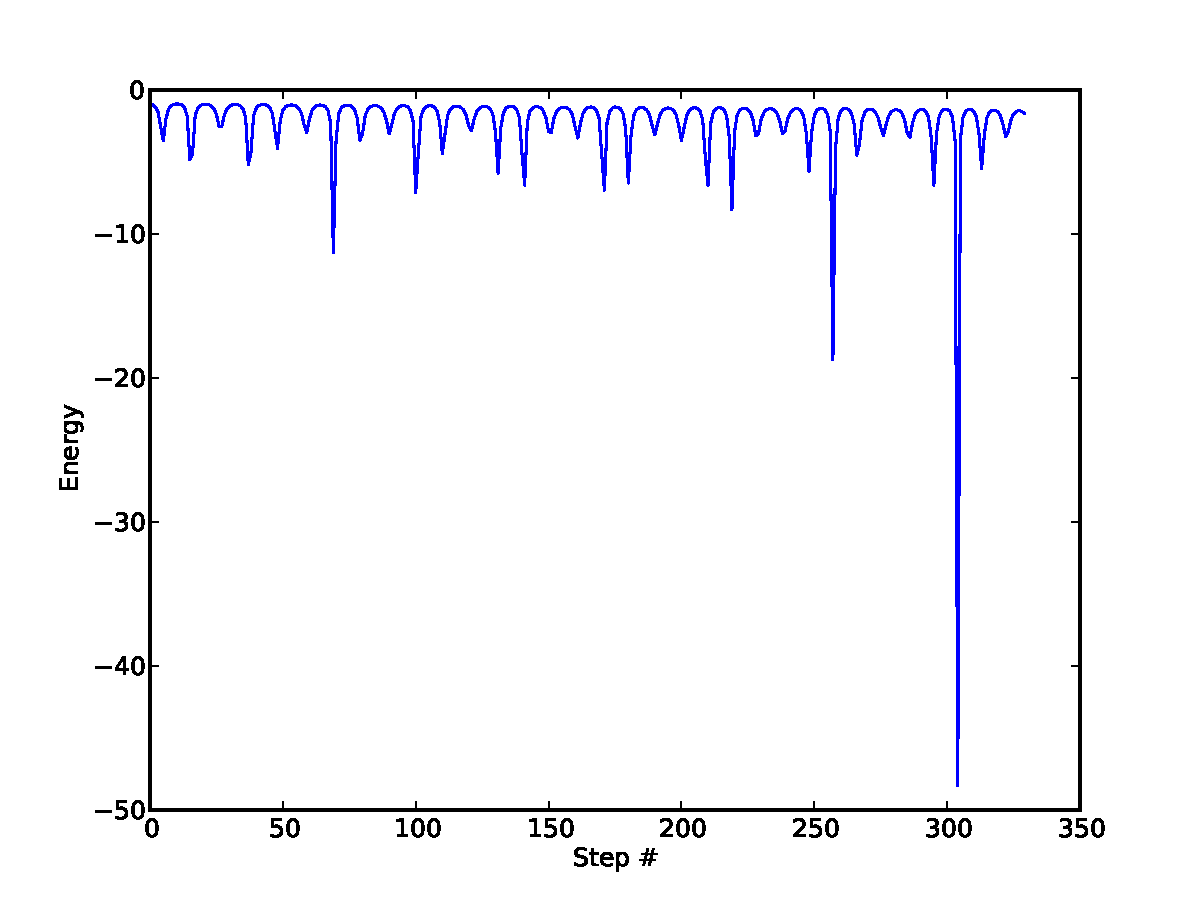
\includegraphics[scale=.7]{E_T_3lf.pdf}
\caption{Energy vs time using leapfrog method and eccentricity=.9.}
\end{center}
\end{figure}

\begin{figure}[h!]
\begin{center}
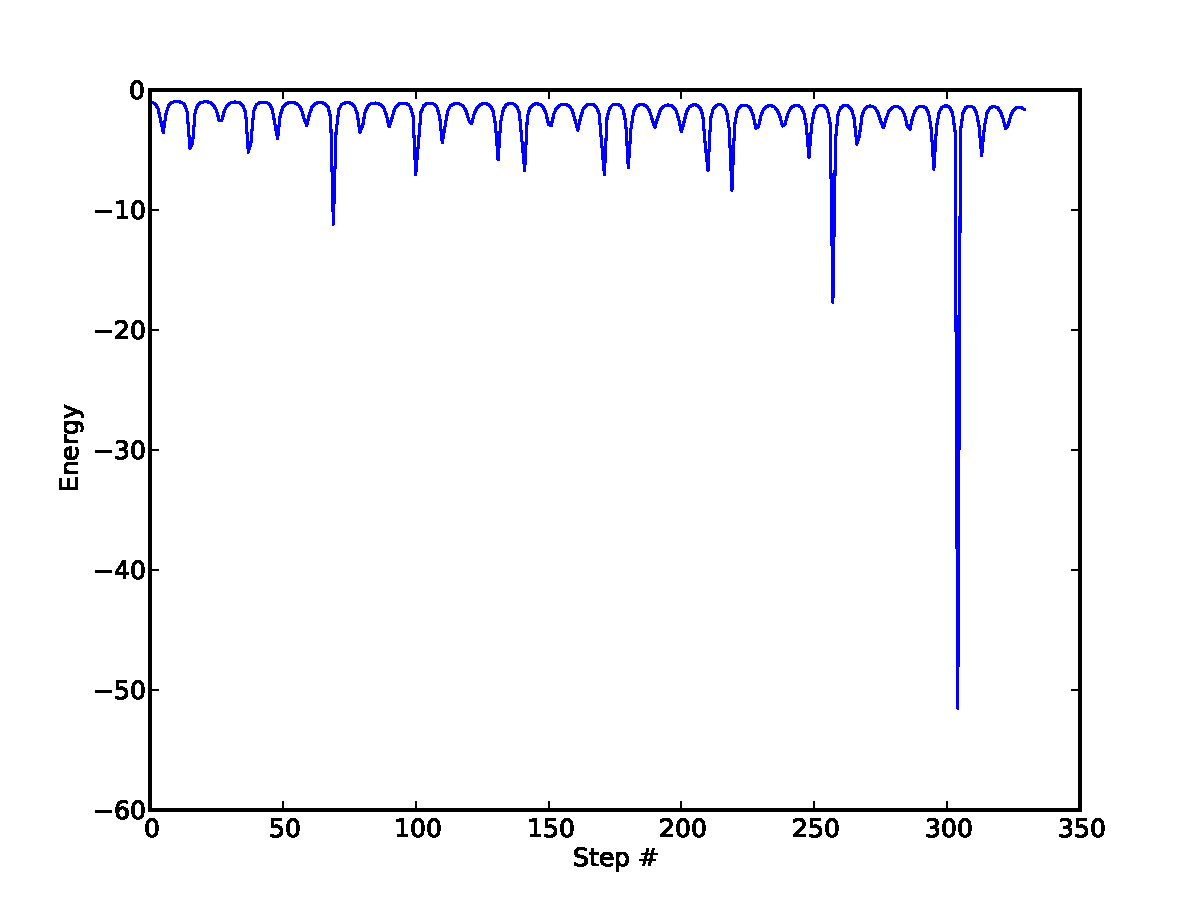
\includegraphics[scale=.7]{E_T_3rk4.pdf}
\caption{Energy vs time using RK4 method and eccentricity=.9.}
\end{center}
\end{figure}

\begin{figure}[h!]
\begin{center}
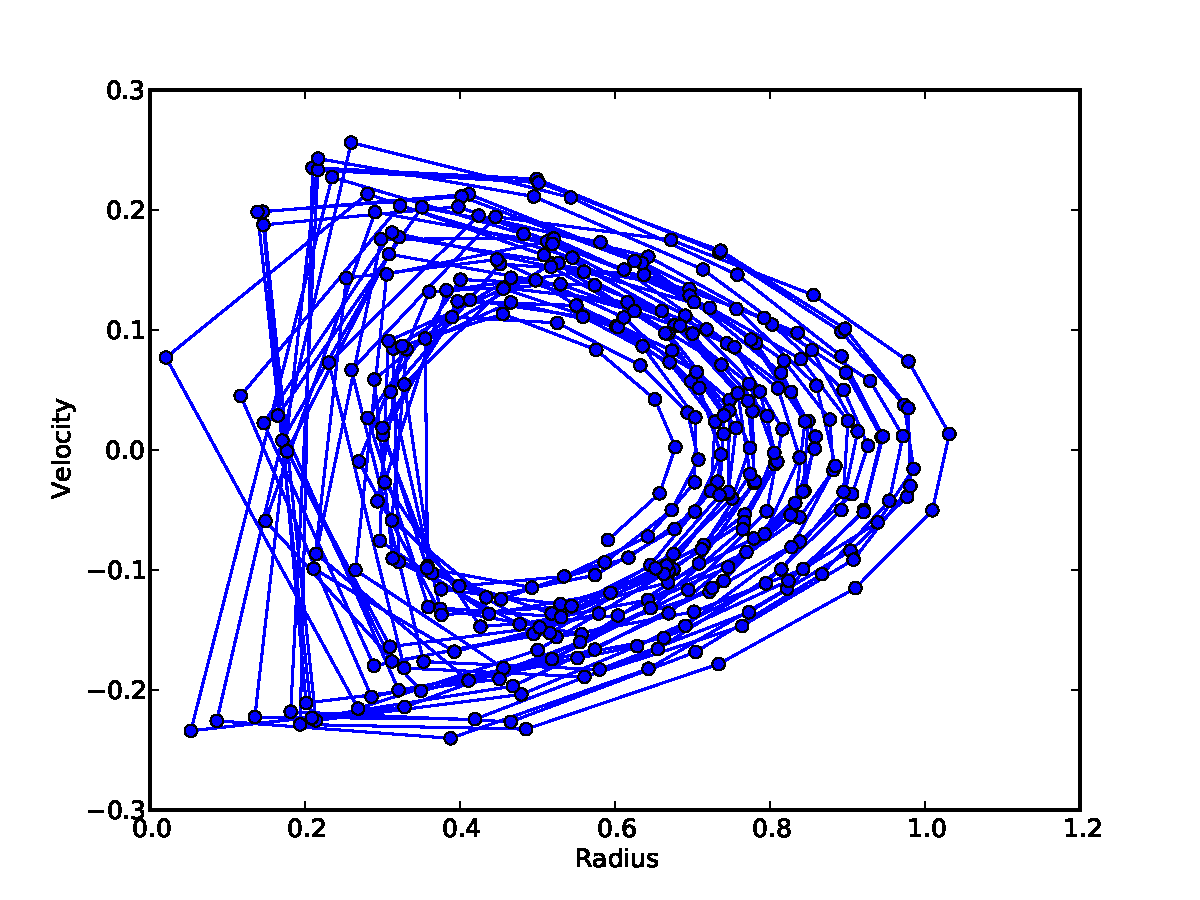
\includegraphics[scale=.7]{R_V_3lf.pdf}
\caption{Phase diagram using leapfrog method and eccentricity=.9.}
\end{center}
\end{figure}

\begin{figure}[h!]
\begin{center}
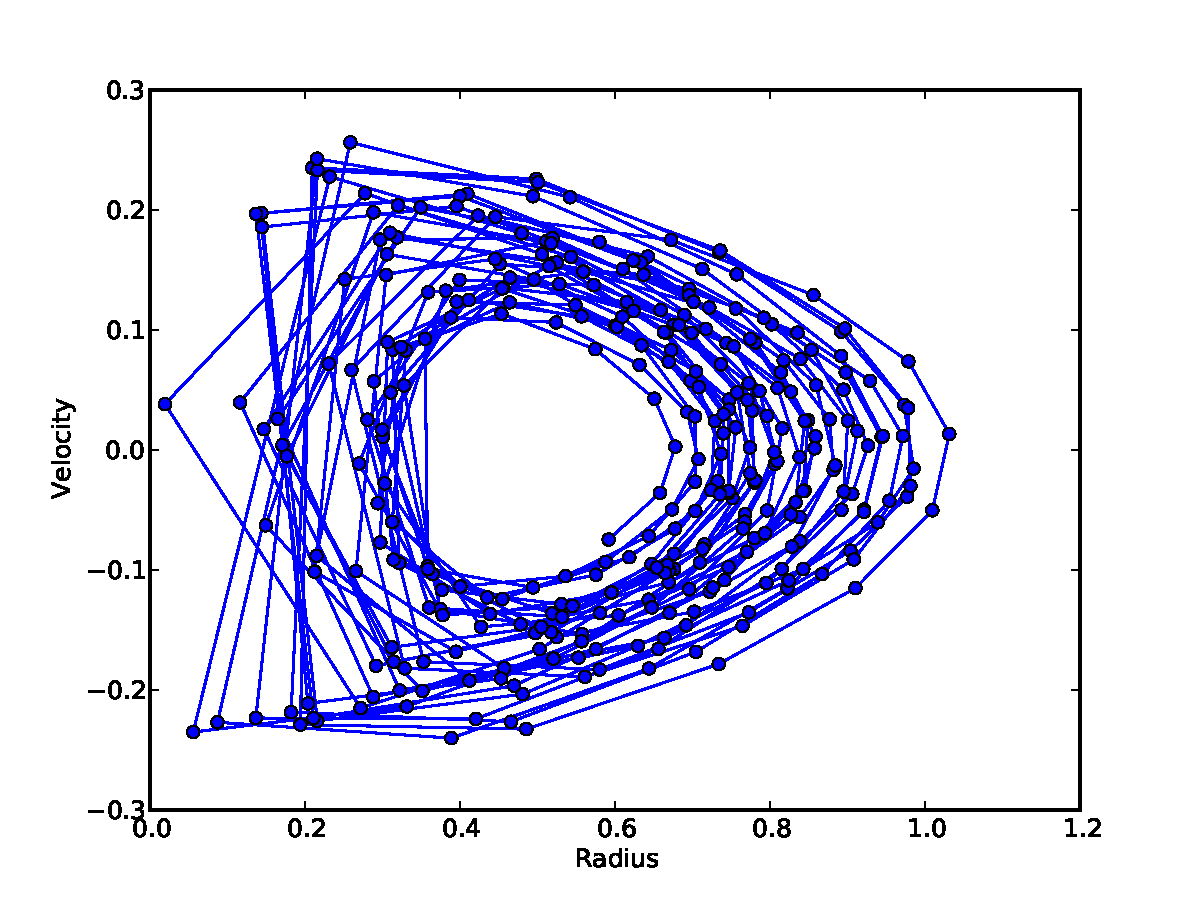
\includegraphics[scale=.7]{R_V_3rk4.pdf}
\caption{Phase diagram using RK4 method and eccentricity=.9.}
\end{center}
\end{figure}

\begin{figure}[h!]
\begin{center}
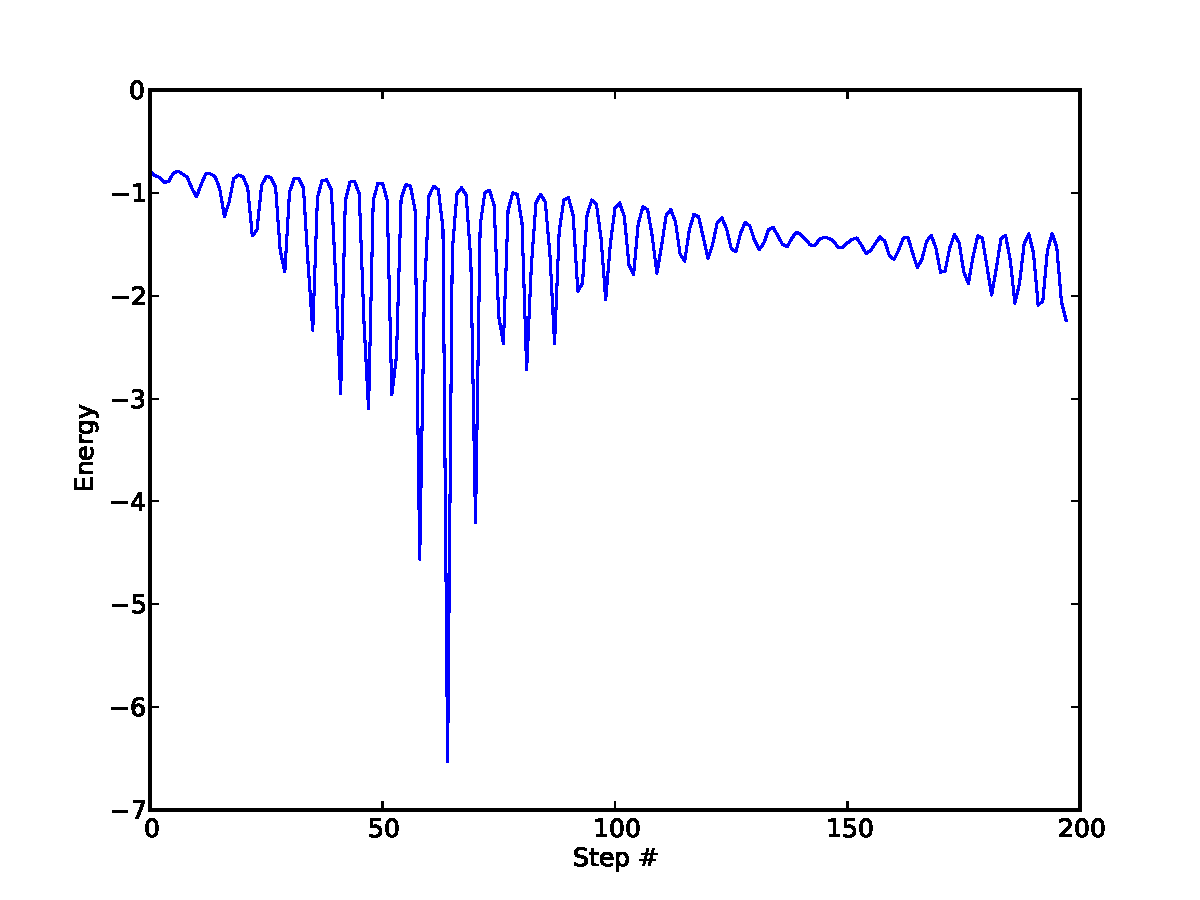
\includegraphics[scale=.7]{E_T_5lf.pdf}
\caption{Energy vs time using leapfrog method and eccentricity=.5.}
\end{center}
\end{figure}

\begin{figure}[h!]
\begin{center}
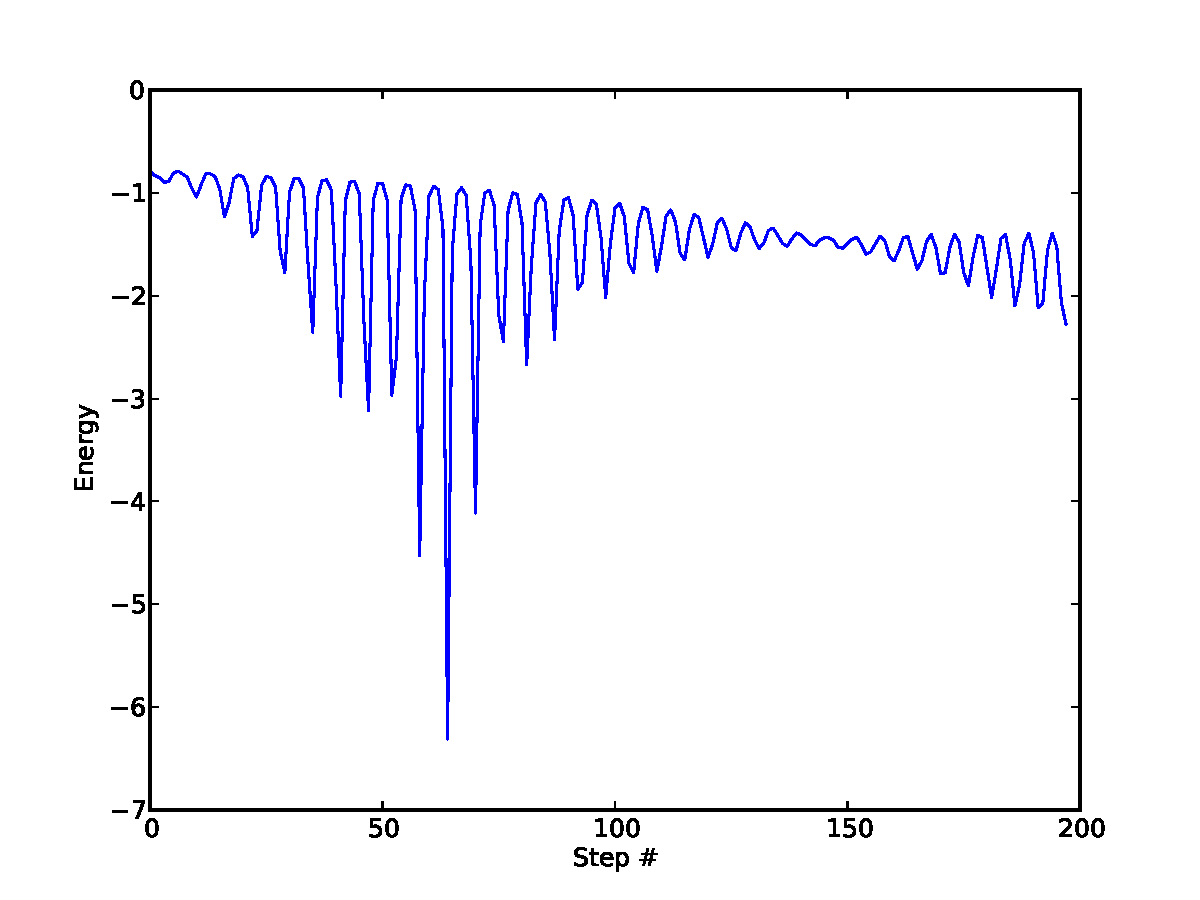
\includegraphics[scale=.7]{E_T_5rk4.pdf}
\caption{Energy vs time using RK4 method and eccentricity=.5.}
\end{center}
\end{figure}

\begin{figure}[h!]
\begin{center}
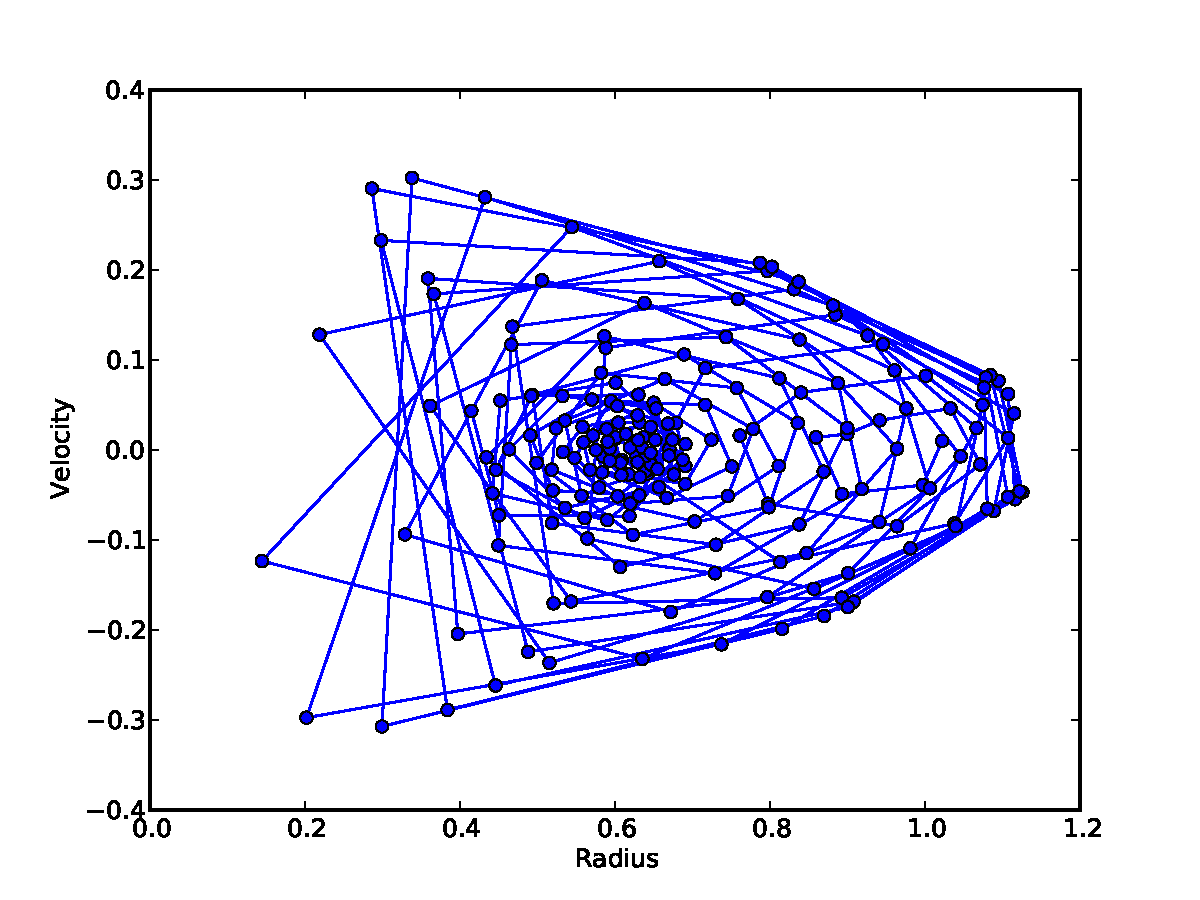
\includegraphics[scale=.7]{R_V_5lf.pdf}
\caption{Phase diagram using leapfrog method and eccentricity=.5.}
\end{center}
\end{figure}

\begin{figure}[h!]
\begin{center}
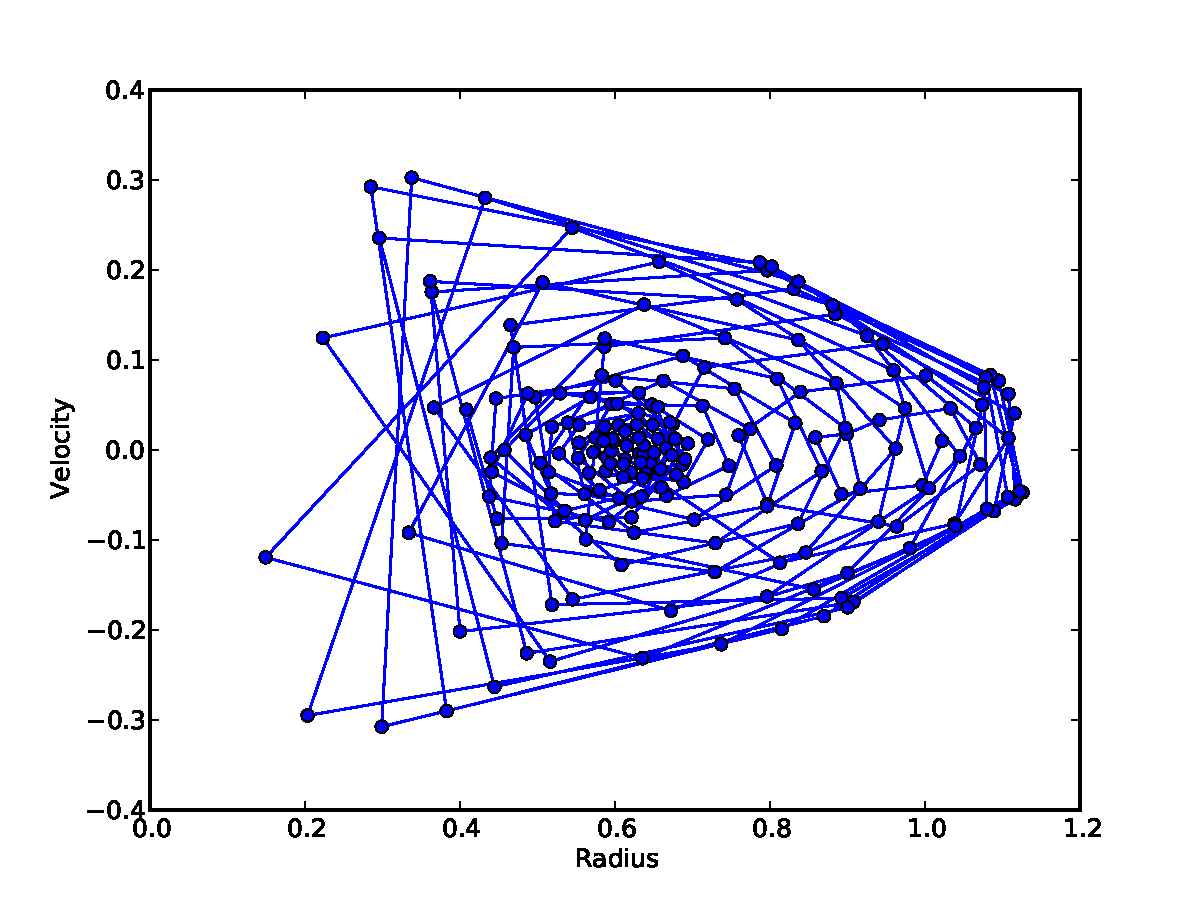
\includegraphics[scale=.7]{R_V_5rk4.pdf}
\caption{Phase diagram using RK4 method and eccentricity=.5.}
\end{center}
\end{figure}
\end{document}
